\documentclass{article}
\usepackage{tikz}
\usepackage{amsmath}

\begin{document}
   To get smooth(non jerky) movement a gradual increase of the velocity is necessary. The stepper motor accelerates and decelerates following a trapezoidal speed profile. Since the stepper motor turns in discrete steps  a algorithm is utilized 
   which can generate the pulses neccesary to approximate the linear increase of the velocity.

   \section{theory}
   \begin{figure}[h]
        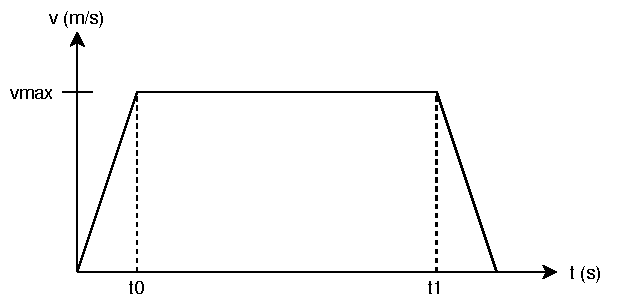
\includegraphics[width=\linewidth]{graph.pdf}
        \caption{Trapezoidal speed profile for the stepper motor.}
        \label{trapezoidal_plot}
   \end{figure}
   As can be seen in figure \ref{trapezoidal_plot}. The idea is that the stepper motor rotate n 
   amount of turns in t seconds with a angular acceleration $\alpha$. For simplicity the acceleration duration and
   deceleration duration are equally as long. In order to fufill these requirements the maximum velocity, $\omega_{max}$, 
   needs to be determined at which the stepper motor rotates. \\

   The paramterization of the trapezoid is given by:
    \[ \omega(t) = \begin{cases} 
          \alpha t & 0 < t \leq t_0 \\
          \alpha t_0 & t_0 < t \leq t_1 \\
          -\alpha(t-t_1) & t_1 < t \leq  \text{stop} 
       \end{cases}
    \]
    By integrating the paremeterization the area is $\theta =\alpha t_0 t_1 = \omega_{max}t_1$ with some algebra formulae for 
    the $t_0$ and $t_1$ can be found:
    \begin{equation}
       t_0 = \frac{w_{max}}{\alpha}, \, \, \, t_1 = \frac{\theta}{w_{max}}
    \end{equation}
    With these equations the total time is given 
    \begin{equation}
      t_{d} = t_0 + t_1
    \end{equation}
    Consequently the maximum velocity can be obtained as function of the total duration, angle and acceleration. Combining equation 1 and 2 
    the following quadratic solution is obtained. 

    \begin{equation}
      \omega_{max}= \frac{\alpha t_d \pm \sqrt{(\alpha t_d)^2 - 4 \alpha \theta}}{2}
    \end{equation}
    but only one of the solutions is valid. 
    \begin{equation}
       N= \frac{1}{\text{gear train} \cdot spr} [\deg^{-1}]
    \end{equation}
    \begin{equation}
         \#\text{steps} = \theta N 
    \end{equation}
    \begin{equation}
       t_0 = \frac{\omega_{max}^2\#steps}{2\theta\alpha}
    \end{equation}
    \begin{equation}
       t_1 = \#\text{steps} - t_0
    \end{equation}
    the anglular velocity is given by the frequency and the step angle. 

    \begin{equation}
       \frac{c}{f} = \Delta t
    \end{equation}
    \begin{equation}
       \omega = \frac{\Delta \theta}{\Delta t} = \frac{\Delta \theta f}{c}
    \end{equation}
    \begin{equation}
       \frac{1}{2}\alpha t^2 = \frac{n}{N}
    \end{equation}
    \begin{equation}
       t = \sqrt{\frac{2n}{\alpha N}}
    \end{equation}
    the difference between to consecutive steps is given by:
    \begin{equation}
      c_n = c_0(\sqrt{n+1}-\sqrt{n})
    \end{equation}
    \begin{equation}
       c_0 = f \sqrt{\frac{2}{\alpha N}}
    \end{equation}
    using taylor series the expression is turned into 
    \begin{equation}
       c_n = c_{n-1} - \frac{2c_{n-1}}{4n+1}
    \end{equation}
    
\end{document}